\documentclass[thesis.tex]{subfiles}

\begin{document}

\iffulldocument\else
	\chapter{KdV5}
\fi

\section{Overview}

A periodic multi-pulse is a multi-modal solution to \cref{eqODE} on a periodic domain. Heuristically, we construct a periodic multi-pulse by gluing together multiple copies of the primary pulse end-to-end in a loop as shown in \cref{fig:permultipulse}.
\begin{figure}
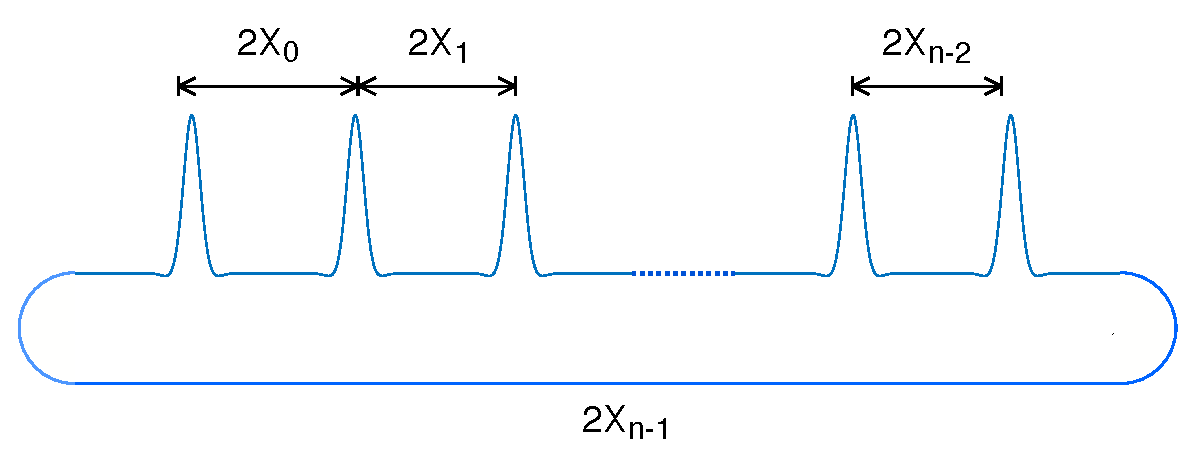
\includegraphics[width=10cm]{periodic/multipulseperiodic}
\caption{Periodic $n-$pulse solution.}
\label{fig:permultipulse}
\end{figure}

In this chapter, we will start by proving the existence of periodic multi-pulses. In the process, we will exhibit a bifurcation structure for periodic 2-pulses. We will then look at their spectral stability.

\section{Existence}

First, we will look at existence. From a spatial dynamics perspective, a periodic multi-pulse is a multi-loop periodic orbit solution $Q_n(x)$ to
\begin{equation}\label{existgenODE}
U'(x) = F(U(x); c)
\end{equation}
which remains close to the primary homoclinic orbit $Q(x)$. A periodic $n$-pulse can be described by $n$ pulse distances $\{X_0, \dots, X_{n-1} \}$, where the distance between consecutive copies of $Q(x)$ in the loop is $2 X_j$. The period of the orbit is $2X$, where $X = X_0 + \dots + X_{n-1}$. A periodic $n$-pulse requires one more pulse distance than an $n$-homoclinic orbit, since we need one more connection to ``close the loop''.  

From a mathematical perspective, rather than describing a periodic multi-pulse by its pulse distances $X_j$, we will adopt an alternative parameterization which is both more convenient and captures the underlying geometry necessary for a periodic $n$-pulse to exist. This parameterization is an adaptation of that in \cite{SandstedeStrut,Sandstede1998} to the periodic case. 

From Hypothesis \ref{hypeqhyp}, the rest state at 0 is a hyperbolic equilibrium point of \cref{existgenODE}. The linearization $DF(0; c)$ about the rest state has a quartet of eigenvalues $\pm \alpha_0 \pm \beta_0 i$, which depends on the wavespeed $c$. All other eigenvalues have real part strictly larger in magnitude than $\alpha_0$. Let
\begin{equation}\label{defrho}
\rho = \frac{\beta_0}{\alpha_0}
\end{equation}
and
\begin{equation}\label{pstar}
p^* = \arctan \rho.
\end{equation}
Define the set
\begin{align}
\mathcal{R} &= \left\{ \exp\left(-\frac{2 k \pi}{\rho}\right) : k \in \N_0 \right\} \cup \{ 0 \},
\end{align}
which is a complete metric space. We will use $r \in \mathcal{R}$ as a scaling parameter. The parameterization is defined as follows.

\begin{definition}\label{def:perparam}
For $n \geq 2$, a \emph{periodic parameterization} of a periodic $n$-pulse is a sequence of parameters $(m_0, \dots, m_{n-1}, \theta)$, where
\begin{enumerate}[(i)]
\item $m_j$ is a nonnegative integer with
\begin{enumerate}
\item at least one of the $m_j \in \{0, 1\}$.
\item $m_{n-1} \geq m_j$ for $j = 0, \dots, n-2$.
\end{enumerate}
\item $\theta \in (\pi + -p^*, p^*]$.
\end{enumerate}
\end{definition}
The selection of $m_{n-1}$ as the largest of the $m_j$ is made only for notational convenience and to allow the parameterization to be unique. Since we are on a periodic domain, there is no loss of generality. The physical pulse distances $X_j$ are determined by these parameters and by the scaling parameter $r$. This works as follows. If $r = \exp\left(-\frac{2 k \pi}{\rho}\right)$, then
\begin{align*}
X_j &= \frac{1}{2 \beta_0}\big( (2 k + m_j)\pi + \theta^*(\theta; m_{n-1} - m_j)\big) + L_0 + \mathcal{O}(r) \\
X_{n-1} &= \frac{1}{2 \beta_0}\big( (2 k + m_{n-1})\pi + \theta \big) + L_0
\end{align*}
where $L_0$ is a constant. The functions $\theta^*(\theta; m): [-\pi + p^*, p^*] \rightarrow \R$ are defined for all nonnegative integers $m$, are continuous in $\theta$, and have the following properties.
\begin{enumerate}[(i)]
\item $\theta^*(0; m) = 0 \text{ for all } m$
\item $|\theta^*(\theta; m)| \leq |\theta|$
\item $|\theta^*(\theta; m)| \leq C \exp\left(-\frac{m \pi}{\rho} \right)$
\item $\theta^*(\theta; 0) = \theta $
\item $\theta^*(p^*; m) = \theta^*(-\pi+p^*; m+1)$ for $m \geq 1$
\end{enumerate}
The last property is a matching condition which ``links up'' the parameterizations corresponding to different $m_j$. These properties, together with the restriction of $\theta$ to the half-open interval $\theta \in (\pi + -p^*, p^*]$, guarantee that each periodic parameterization corresponds to a unique periodic multi-pulse (up to cyclic permutations of the $m_j$; see \cref{remark:cyclicperm} below). The proof that the functions $\theta^*(\theta; m)$ exist and have these properties is given in Lemma \ref{thetaparamlemma} below. [A PICTURE WOULD DO WELL HERE.]

We can now state the main theorem of this section, which gives conditions for the existence of periodic multi-pulses. The requirement that the scaling parameter $r$ be sufficiently small means that the individual pulses must be well-separated. 

\begin{theorem}[Existence of $n$-periodic solutions]\label{perexist}
Assume Hypotheses \ref{Ehyp}, \ref{Hhyp}, \ref{hypeqhyp}, \ref{Qexistshyp}, and \ref{H0transversehyp}. Let $Q(x)$ be the transversely constructed, symmetric primary pulse solution to \eqref{genODE} from Hypothesis \ref{Qexistshyp}. For any periodic parameterization $(m_0, \dots, m_{n-1}, \theta)$ with $\theta \notin \{-\pi + p^*, p^* \}$, there exists $r_* = r^*(m_0, \dots, m_{n-1}, \theta) \in \mathcal{R}$ with $r_* > 0$ such that for any $r \in \mathcal{R}$ with $r \leq r_*$:
\begin{enumerate}[(i)]
	\item There exists a periodic $n$-pulse solution $Q_n(x) = Q_n(x; m_0, \dots, m_{n-1}, \theta, r)$ to \eqref{genODE}.

	\item The distances between consecutive copies of $Q(x)$ are $2X_j$, where
	\begin{align}\label{Xj}
		X_j(r; m_j, m_{n-1},\theta) &= \frac{1}{2 \alpha_0} |\log r| + \frac{1}{2\beta_0} t_j(r; m_j,m_{n-1}, \theta) + L_0 && j = 0, \dots, n-2 \\
		X_{n-1}(r; m_{n-1}, \theta) &= \frac{1}{2 \alpha_0} |\log r| + \frac{1}{2 \beta_0}\big( m_{n-1}\pi + \theta \big) + L_0.
	\end{align}
	The $t_j(r; m_j, m_{n-1}, \theta): \mathcal{R} \rightarrow \R$ are smooth functions with 
	\[
	t_j(0; m_j, \theta) = m_j \pi + \theta^*(\theta; m_{n-1} - m_j),
	\]
	and $L_0$ is a constant.

	\item The periodic domain has length $2X$, where
	\begin{align}\label{Xdomain}
	X(r; m_0, \dots, m_{n-1}, \theta) = \frac{n}{2\alpha_0} |\log r| + \frac{1}{2\beta_0} \sum_{j=0}^{n-1} t_j(r; m_j, \theta) + n L_0
	\end{align}

	\item $Q_n(x)$ can be written as piecewise perturbation of the primary pulse $Q(x)$. Details are given below in Lemma \ref{solvewithjumps}.
\end{enumerate}
\end{theorem}

\begin{remark}\label{remark:cyclicperm}
The periodic $n$-pulses constructed in \cref{perexist} are unique up to ``rotation'' of the integers $(m_0, \dots, m_{n-1})$ in the periodic parameterization. For example, $(m_0, m_1, m_2, \theta)$, $(m_2, m_0, m_1, \theta)$, and $(m_1, m_2, m_0, \theta)$ all give the same solution.
\end{remark}

The condition that $\theta \notin \{-\pi + p^*, p^*) \}$ in \cref{perexist} is used to avoid any bifurcation points which may arise in the construction. For periodic 2-pulses, we can use a symmetry argument to give a complete bifurcation picture. In the next theorem, we state an existence result for periodic 2-pulses and show that asymmetric solutions bifurcate from symmetric solutions in a series of pitchfork bifurcations. We note that for the symmetric periodic 2-pulses we are using a different parameterization than in \cref{perexist}.

\begin{theorem}\label{2pulsebifurcation}
Assume Hypotheses \ref{Ehyp}, \ref{Hhyp}, \ref{hypeqhyp}, \ref{Qexistshyp}, and \ref{H0transversehyp}. Let $Q(x)$ be a transversely constructed, symmetric primary pulse solution to \eqref{genODE}.

There exists $r_* \in \mathcal{R}$ with $r_* > 0$ such that for all $r \leq r_*$ and $m_0 \in \{0, 1\}$
\begin{enumerate}[(i)]
	\item There exists a family of symmetric periodic 2-pulses $\tilde{Q}_2(x; m_0, s_0, r)$ parameterized by $s_0 \in [0, \pi)$. The distances $\tilde{X}_j$ are given by
	\begin{equation}\label{2psymmdist}
		\tilde{X}_0(r, s_0) = \tilde{X}_1(r, s_0) = \frac{1}{2 \alpha_0} |\log r| + \frac{\pi}{2\beta_0} (m_0 + s_0) + L_0.
	\end{equation}
	\item There exists a family of asymmetric periodic 2-pulses $Q_2(x; m_0, s_1, r)$ with distances $X_1 > X_0$ parameterized by $s_1 \in [p^*, \infty)$. The distances $X_j$ are given by
	\begin{equation}\label{2pasymmdist}
	\begin{aligned}
		X_0(r, m_0, s_1) &= \frac{1}{2 \alpha_0} |\log r| + \frac{1}{2\beta_0} t_0(r; m_0, s_1) + L_0 \\
		X_1(r, s_1) &= \frac{1}{2 \alpha_0} |\log r| + \frac{1}{2\beta_0} s_1 + L_0, 
	\end{aligned}
	\end{equation}
	where $t_0(r; m_0, s_1)$ is smooth in $r$, continuous in $t_1$, and $t_0(0; m_0, k \pi) = m_0$ for all nonnegative integers $k$. Furthermore,
	\begin{align}\label{deft0}
	t_0(0; m_0, s_1) = m_0 \pi + \mathcal{O}\left(-\frac{1}{\rho} s_1 \right)
	\end{align}
	The periodic domain has length $2X$, where
	\begin{equation}\label{X2pdomain}
	X(r, m_0, s_1) = \frac{1}{2 \alpha_0} 2 |\log r| + \frac{1}{2\beta_0} \left( t_0(r; m_0, s_1) + s_1\right) + 2 L_0.
	\end{equation}

	\item The two families meet at a pitchfork bifurcation. In terms of the two parameterizations, this occurs when $s_0 = p^*(m_0; r)$ and $s_1 = p^*$. The bifurcation points $p^*(m_0; r)$ are smooth in $r$, and
	\[
	p^*(m_0; r) \rightarrow \arctan \rho \text{ as }r \rightarrow 0.
	\]
\end{enumerate}
\end{theorem}
[THIS NEEDS A NICE PICTURE.]

\section{Spectral stability}

In this section, we look at the spectral stability of the periodic multi-pulses which we constructed in the previous section. To do this, we will adapt the framework we set up in \cref{sec:genspectrum}.

Let $Q(x)$ be the primary pulse solution. Let $Q_n(x)$ be any periodic multi-pulse solution constructed according to Theorem \ref{perexist}, and let $X$ be given by \cref{Xdomain}. Let $q_n(x)$ be the first component of $Q_n(x)$. We are interested in the PDE eigenvalue problem
\begin{equation}\label{genPDEeigper}
\partial_x \calL(q_n) v = \lambda v
\end{equation}
resulting from the linearization of the original PDE \cref{genPDE} about $q_n(x)$. It is natural to pose \cref{genPDEeigper} on the space of periodic functions $H^{2m}_{\text{per}}[-X,X]$, where
\[
H^{2m}_{\text{per}}[-X,X] = \left\{ f \in H^{2m}(\R) : f^{(k)}(-X) = f^{(k)}(X) \text{ for } k = 0, \dots, 2m \right\} 
\]
The norm on this space is the $H^{2m}$ norm restricted to $[-X, X]$. 

As in \cref{sec:genspectrum}, we use a spatial dynamics formulation and write the PDE eigenvalue problem \cref{genPDEeigper} as the first order system of ODEs
\begin{equation}\label{PDEeigsystemper2}
\begin{aligned}
V'(x) &= A(Q_n(x))V(x) + \lambda B V(x) \\
V(-X) &= V(X)
\end{aligned}
\end{equation}
where $V(x) \in C^0(\R,\R^{2m+1})$, and we have imposed an additional periodic constraint on $V(x)$. To aid in the analysis, we rewrite \cref{PDEeigsystemper2} as
\begin{equation}\label{PDEeigsystemper3}
\begin{aligned}
V'(x) &= A(Q_n(x); \lambda)V(x) \\
V(-X) &= V(X),
\end{aligned}
\end{equation}
where $A(Q_n(x); \lambda) = A(Q_n(x)) + \lambda B$. Let $A(\lambda) = A(0; \lambda)$. By Lemma \ref{eigA0lemma}, $A(0)$ has a simple eigenvalue at 0. The next lemma states that for small $\lambda$, $A(\lambda)$ has a simple eigenvalue $\nu(\lambda)$ near 0; it is proved as part of Lemma \ref{nulambdalemma} below.

% nu(lambda) lemma
\begin{lemma}\label{nulambdalemmasimple}
There exists $\delta_0 > 0$ such that for $|\lambda| < \delta_0$, the matrix $A(\lambda)$ has a simple eigenvalue $\nu(\lambda)$ near 0.
\end{lemma}

We can now state the main theorem of this section, which provides a condition for \cref{PDEeigsystemper3} to have a solution. Since the spatial dynamics formulation \cref{PDEeigsystemper3} is equivalent to the PDE eigenvalue problem, this allow us to find the eigenvalues of \cref{genPDEeigper}. This theorem is analogous to \cite[Theorem 2]{Sandstede1998}, where the matrix $S(\lambda)$ is replaced by a block matrix.

% block matrix theorem
\begin{theorem}\label{blockmatrixtheorem}
Assume Hypotheses \ref{Ehyp}, \ref{Hhyp}, \ref{hypeqhyp}, \ref{Qexistshyp}, and \ref{H0transversehyp}, and \ref{Melnikov2hyp}. Let $Q(x)$ be the primary pulse solution, and let $\Psi(x)$ be the solution to the adjoint variational equation from Lemma \ref{varadjsolutions}. Choose any periodic parameterization $(m_0, \dots, m_{n-1}, \theta)$ with $\theta \neq \pm \pi$, and let $r_*$ be as in \cref{perexist}. 

Choose any positive integer $N$. Then for any $r \leq r_*$ there exists $\delta(r,N)$, where $0 < \delta(r,N) < N/|\log r|$, with the following property. There exists a bounded, nonzero solution $V(x)$ of \cref{PDEeigsystemper3} for $|\lambda| < \delta(r,N)$ if and only if
\begin{equation}\label{blockmatrixcond}
E(\lambda) = \det S(\lambda) = 0.
\end{equation}
$S(\lambda)$ is the $(2n \times 2n)$ block matrix
\begin{equation}\label{blockeq}
S(\lambda) = 
\begin{pmatrix}
K(\lambda) + C_1 & \lambda K_1(\lambda) + D_1 \\
-\lambda M^c K^+(\lambda) C_2 & A - \lambda^2 MI + D_2
\end{pmatrix}
\end{equation}
The individual terms in $S(\lambda)$ are as follows.

\begin{enumerate}
\item $K(\lambda)$ is the banded matrix
\begin{equation}
K(\lambda) = 
\begin{pmatrix}
e^{-\nu(\lambda)X_1} & & & & & -e^{\nu(\lambda)X_0} \\
-e^{\nu(\lambda)X_1} & e^{-\nu(\lambda)X_2} \\
& -e^{\nu(\lambda)X_2} & e^{-\nu(\lambda)X_3} \\
& \ddots & \ddots & &&  \\
& & & & -e^{\nu(\lambda)X_{n-1}} & e^{-\nu(\lambda)X_0} 
\end{pmatrix}
\end{equation}
where $\nu(\lambda)$ is defined in Lemma \ref{nulambdalemmasimple}. $K^+(\lambda)$ is the same matrix with all terms positive.

\item $A$ is the symmetric banded matrix
\begin{align}\label{Asymm}
A &= \begin{pmatrix}
-a_0 -a_1 & a_0 + a_1 \\
a_0 + a_1 & -a_0 - a_1
\end{pmatrix} && n = 2 \\
A &= \begin{pmatrix}
-a_{n-1} - a_0 & a_0 & & &  & a_{n-1}\\
a_0 & -a_0 - a_1 &  a_1 \\
& a_1 & -a_1 - a_2 &  a_2 \\
& \ddots & \ddots & \ddots \\
a_{n-1} & & & & a_{n-2} & -a_{n-2} - a_{n-1} \\
\end{pmatrix} && n > 2 \nonumber
\end{align}
where
\begin{align*}
a_i &= \langle \Psi(X_i), Q'(-X_i) \rangle
\end{align*}

\item $K_1(\lambda)$ is the matrix
\begin{align*}
K_1(\lambda) &= \begin{pmatrix}
s_0^+ - s_1^- & s_1^- &&& -s_0^+ \\
-s_1^+ & s_1^+ - s_2^- & s_2^- \\
& -s_2^+ & s_2^+ - s_3^- & s_3^- \\ && \ddots \\
\\
s_0^- &&& -s_{n-1}^+ & s_{n-1}^+ - s_0^- 
\end{pmatrix}
\end{align*}
with entries
\begin{align*}
s_i^- &= e^{-\nu(\lambda)X_i} q(X_i)\\
s_i^+ &= e^{\nu(\lambda)X_i} q(X_i)\\
\end{align*}
where $q(x)$ is the first component of the primary pulse solution $Q(x)$. 

\item $M$ and $M^c$ are the Melnikov-type integrals
\begin{align*}
M &= \int_{-\infty}^\infty q(y) \partial_c q(y) dy \\
M^c &= \int_{0}^\infty q(y) v^c(y) dy
\end{align*}
where $v^c(y)$ is the first component of $V^c(y)$, which is defined in \cref{varadjsolutions}.

\item The remainder matrices and $K_1(\lambda)$ are analytic in $\lambda$ and have uniform bounds
\begin{align*}
|K_1(\lambda)| &\leq C r^{1/2} \\
|C_1| &\leq C |\lambda|(|\lambda| + r^{1/2}) \\
|D_1| &\leq C |\lambda|(|\lambda| + r^{1/2})^2 \\
|C_2| &\leq C (|\lambda| + r^{1/2})^2 \\
|D_2| &\leq C (|\lambda| + r^{1/2})^3 
\end{align*}
The constants $C$ depend on $N$.
\end{enumerate}
\end{theorem}

To leading order, equation \cref{blockeq} is block diagonal with blocks $A - \lambda^2 MI$ and $K(\lambda)$. As in \cref{chapter:kdv5homoclinic}, we expect that points where $A - \lambda^2 MI$ is singular will give us interaction eigenvalues as well as two kernel eigenvalues. In addition, we expect to find another set of eigenvalues at the points where $K(\lambda)$ is singular, which are
\begin{align*}
\lambda &= c\frac{k \pi i}{X} && k \in \Z.
\end{align*}
This will be a set of discrete, purely imaginary eigenvalues (which will include one more kernel eigenvalue). Since these are the periodic analogue of the essential spectrum in the $n$-homoclinic case, we will refer to these as essential spectrum eigenvalues, even though they are technically still part of the point spectrum. 

\begin{remark}
For any positive integer $N$ we choose, it follows from \cref{Xdomain} that for all $r \leq r_*$,
\begin{align*}
\left| c\frac{k \pi i}{X} \right| \leq \delta(r,N) && k \in \Z, |k|\leq N.
\end{align*}
Thus the restriction $\delta(r,N) < N/|\log r|$ in \cref{blockmatrixtheorem} will not hinder a search for the first $N$ essential spectrum eigenvalues.
\end{remark}

\section{Spectrum of periodic 2-pulse}

We will first consider the simplest case, which is the periodic 2-pulse. For this case, the block matrix  $S(\lambda)$ from \cref{blockmatrixtheorem} is a $4\times4$ matrix. With the aid of Mathematica, we can compute its determinant.

\begin{corollary}\label{2blockmatrix}
For a periodic 2-pulse, $E(\lambda)$ from \cref{blockmatrixtheorem} is given by
\begin{equation}\label{2detBeq}
\begin{aligned}
E(\lambda) &= \left(-2 \lambda^2 M (2a + \lambda^2 M) + R_1 \right) \sinh(\nu(\lambda)X) \\
&-4 M M^c \lambda^4 ( q(X_0) \sinh(\nu(\lambda)X_0) + q(X_1) \sinh(\nu(\lambda)X_1) ) \cosh(\nu(\lambda)X)  + R_2
\end{aligned}
\end{equation}
where
\begin{equation}\label{2pa}
a = \langle \Psi(X_0), Q'(-X_0) \rangle + \langle \Psi(X_1), Q'(-X_1) \rangle
\end{equation}
and the remainder terms have bounds
\begin{align*}
|R_1| \leq C(r^{1/2} + |\lambda|)^5 \\
|R_2| \leq C(r^{1/2} + |\lambda|)^6
\end{align*}
\end{corollary}

The interaction eigenvalue pattern will be determined by the quantity $a$ in \cref{2pa}. We characterize this in the next lemma.

\begin{lemma}\label{lemma:chara}
Let $r_*$ be as in Theorem \ref{2pulsebifurcation}. Then for any $r \leq r_*$:
\begin{enumerate}[(i)]
	\item For a symmetric periodic 2-pulse $\tilde{Q}_2(x; m_0, s_0, r)$, $a = r \tilde{a}(r; m_0, s_0)$, where $\tilde{a}(r; m_0, s_0)$ is smooth in $r$. For $m_0 = 0$,
	\begin{equation}
	\begin{aligned}
	\tilde{a}(0; m_0, s_0) &= 0 && \text{if }s_0 = p^* \\
	\tilde{a}(0; m_0, s_0) &> 0 && \text{if }s_0 < p^* \\
	\tilde{a}(0; m_0, s_0) &< 0 && \text{if }s_0 > p^*
	\end{aligned}
	\end{equation}
	These are reversed for $m_0 = 1$.
	\item For an asymmetric periodic 2-pulse $Q_2(x; m_0, s_1, r)$, $a = r \tilde{a}(r; m_0, s_1)$, where $\tilde{a}(r; m_0, s_1)$ is smooth in $r$ and continuous in $s_1$. For all $s_1 > -\pi + p^*$,
	\begin{equation}
	\begin{aligned}
	\tilde{a}(0; m_0, s_1) &< 0 && \text{if }m_0 = 0 \\
	\tilde{a}(0; m_0, s_1) &> 0 && \text{if }m_0 = 1
	\end{aligned}
	\end{equation}
	Furthermore,
	\begin{equation}\label{tildeas1limit}
	\tilde{a}(0; m_0, s_1) = \tilde{a}^*(m_0) + \mathcal{O}\left( e^{-\frac{1}{\rho}s_1} \right),
	\end{equation}
	where $\tilde{a}^*(m_0) < 0$ if $m_0 = 0$ and $\tilde{a}^*(m_0) > 0$ if $m_0 = 1$.
\end{enumerate}	
\end{lemma}
AS OF NOW I ONLY HAVE A COMPLETE PROOF FOR PART (i) AND FOR \cref{tildeas1limit}.

\subsection{Non-interfering essential spectrum }

First, we will consider the case where the interaction eigenvalues are ``out of the way'' of the essential spectrum eigenvalues. Since the interaction eigenvalues scale like $r^{1/2}$ and the essential spectrum eigenvalues scale like $1/|\log r|$, we can always choose $r$ sufficiently small so that this occurs. We expect that the eigenvalues will come in one of the two patterns shown in \cref{fig:2ppatterns}.

\begin{figure}
\begin{center}
\begin{tabular}{cc}
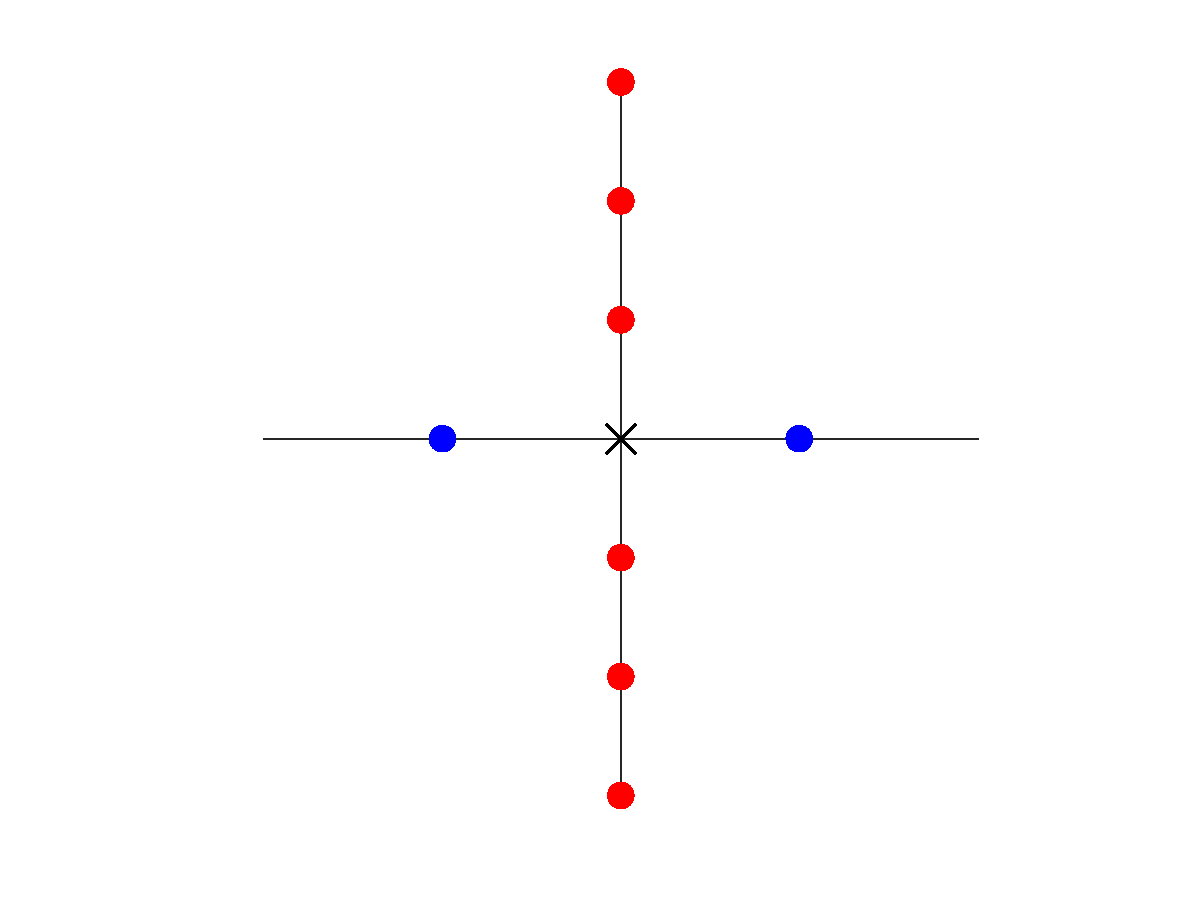
\includegraphics[width=5cm]{images/kdv5/2punstableeigpattern.eps} &
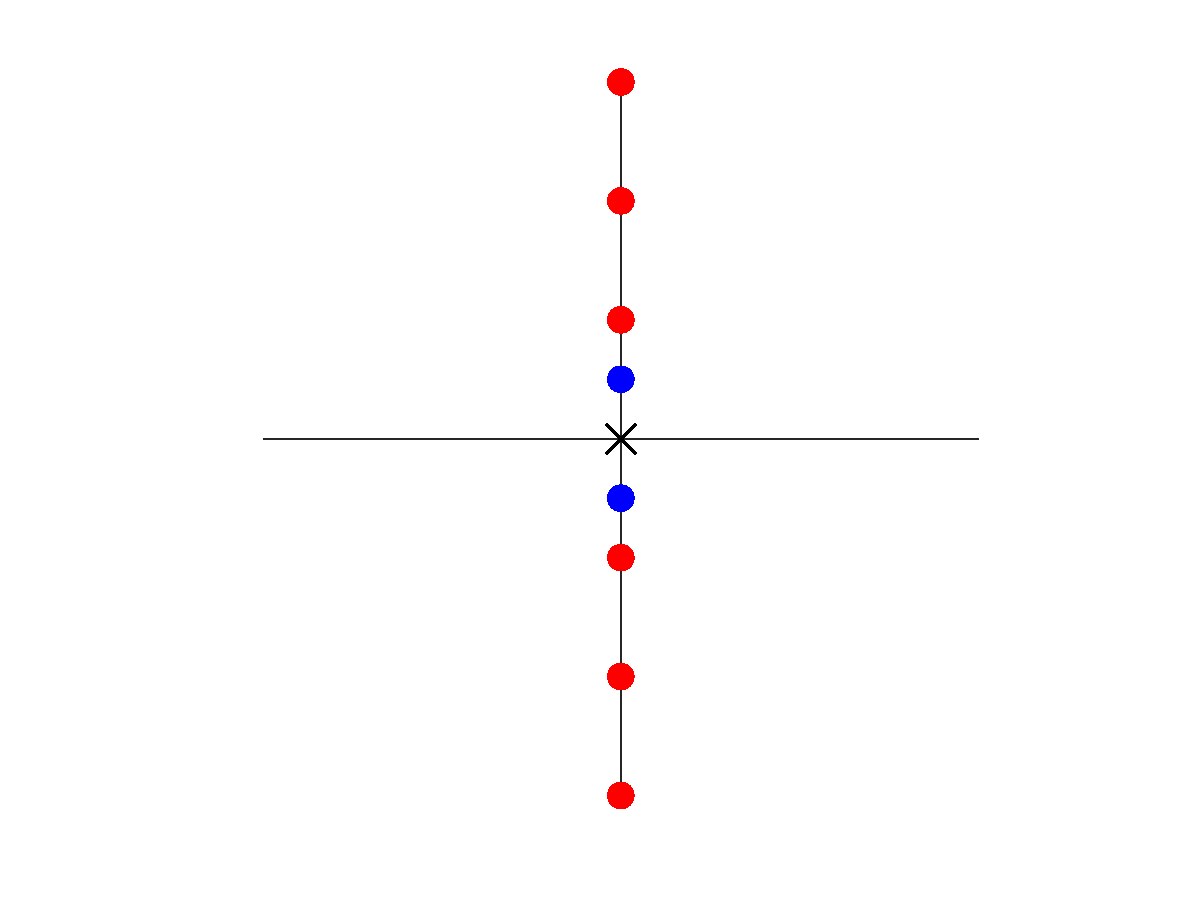
\includegraphics[width=5cm]{images/kdv5/2pstableeigpattern.eps} 
\end{tabular}
\caption{Eigenvalue patterns for periodic 2-pulse with essential spectrum out of the way. Blue dots are interaction eigenvalues, red dots are essential spectrum eigenvalues, and black X at the origin represents the three kernel eigenvalues. Left panel shows a pair of real interaction eigenvalues, and right panel shows a pair of purely imaginary interaction eigenvalues. }
\label{fig:2ppatterns}
\end{center}
\end{figure}

We will state the result separately for asymmetric and symmetric periodic 2-pulses. First, we locate the eigenvalues for asymmetric 2-pulses. As long as $r$ is chosen sufficiently small, the interaction eigenvalue pattern is determined by the parameter $m_0$, and the essential spectrum eigenvalues do not interfere.

\begin{theorem}\label{theorem:2peigsassym}
Assume Hypotheses \ref{Ehyp}, \ref{Hhyp}, \ref{hypeqhyp}, \ref{Qexistshyp}, \ref{H0transversehyp}, \ref{Melnikov2hyp}. Let $r_*$ be as in \cref{2pulsebifurcation}. Let $\tilde{a}(r)$ be as in \cref{lemma:chara}. Choose any integer $N > 0$, and let $\delta(N,r)$ be as in Theorem \ref{blockmatrixtheorem}. Then for every $m_0 \in \{0, 1\}$ and $s_1 > -\pi + p^*$ there exists $r_1 = r_1(m_0, s_1, N) \leq r_*$ with the following property. For any $r \leq r_1$, the following hold regarding the spectrum associated with the asymmetric periodic 2-pulse $Q_2(x; m_0, s_1, r)$.

\begin{enumerate}[(i)]
\item There is an eigenvalue at 0 with algebraic multiplicity 3. 
\item Let $N_1 \leq N$ be the largest positive integer such that $N_1/|\log r| < \delta(N,r)$. Then there are $2N_1$ nonzero essential spectrum eigenvalues $\lambda = \{ \pm \lambda_m^{\text{ess}} : m = 1, \dots, N_1 \}$, where
\[
\lambda_m^{\text{ess}}(r) = c \frac{m \pi i}{X}+  \mathcal{O}\left( \frac{1}{|\log r|^2} \right)
\]
is on the imaginary axis and $X$ is given by \cref{Xdomain}.

\item There is a pair of interaction eigenvalues located at
	\begin{align*}
	\lambda^{\text{int}}(r) = \pm \left( \sqrt{-\frac{2 \tilde{a}(r)}{M}}r^{1/2} + \mathcal{O}\left( r \right) \right)
	\end{align*}
with $|\lambda^{\text{int}}(r)| < \frac{1}{2}|\lambda_1^{\text{ess}}(r)|$. If $M > 0$, these are real when $m_0 = 0$ and purely imaginary when $m_0 = 1$. (This is reversed if $M < 0)$. 
\item There are no other eigenvalues inside a circle with radius slightly larger than $|\lambda_{N_1}^{\text{ess}}(r)|$.
\end{enumerate}
\end{theorem}

Next, we consider the symmetric periodic 2-pulse. As long as we are away from the pitchfork bifurcation points, i.e. as long as $\tilde{a}(0) \neq 0$, the results of \cref{theorem:2peigsassym} hold in the symmetric case as well; the only difference is that the eigenvalue pattern is determined by the sign of $\tilde{a}_0(0)$ rather than by $m_0$. Thus we only need to consider what happens at the pitchfork bifurcation point.

\begin{theorem}\label{theorem:2peigssym}
Assume Hypotheses \ref{Ehyp}, \ref{Hhyp}, \ref{hypeqhyp}, \ref{Qexistshyp}, \ref{H0transversehyp}, \ref{Melnikov2hyp}. Let $r_*$ be as in \cref{2pulsebifurcation}. Then there exists $r_1 \leq r_*$ such that for all $r \leq r_1$ and for $m_0 \in \{0, 1\}$, there is eigenvalue at 0 with algebraic multiplicity 5 for the symmetric periodic 2-pulse $\tilde{Q}_2(x; m_0, p^*(r), r)$.
\end{theorem}

\subsection{Krein bubble}

We now consider what happens when a purely imaginary interaction eigenvalue is close to an essential spectrum eigenvalue. We will show that under certain conditions, an instability bubble forms when an essential spectrum eigenvalue (positive Krein signature) collides with an interaction eigenvalue (negative Krein signature) on the imaginary axis. From \cref{theorem:2peigsassym}, we can always choose $r$ sufficiently small so that this does not occur. In addition, it can never occur for a symmetric 2-pulse. 

Before we state the theorem, we will illustrate what occurs graphically. Let $\lambda_*$ be the imaginary interaction eigenvalue in the upper half-plane, and let $\lambda_1$ be the first essential spectrum eigenvalue. Let $t \in [-2, 2]$ be a dimensionless parameter which measures the distance between $\lambda_1$ and $\lambda_*$. Let $R_0$ be a parameter that depends the primary pulse and on intrinsic properties of the system. We will show that if $R_0 > 0$ (which can be checked numerically), a Krein bubble occurs. Specifically, there is a pair of eigenvalues $\lambda_{1,2}$ near $\lambda_*$ which can be parameterized by $t$. As $t$ decreases from $2$ to $-2$, a pair of purely imaginary eigenvalues collides, moves off of the imaginary axis, travels on a circle centered at $\lambda_*$, and then recombines. This is illustrated in \cref{fig:kreinbubbles}. Results from numerical analysis match this picture.
\begin{figure}
\begin{center}
\begin{tabular}{ccc}
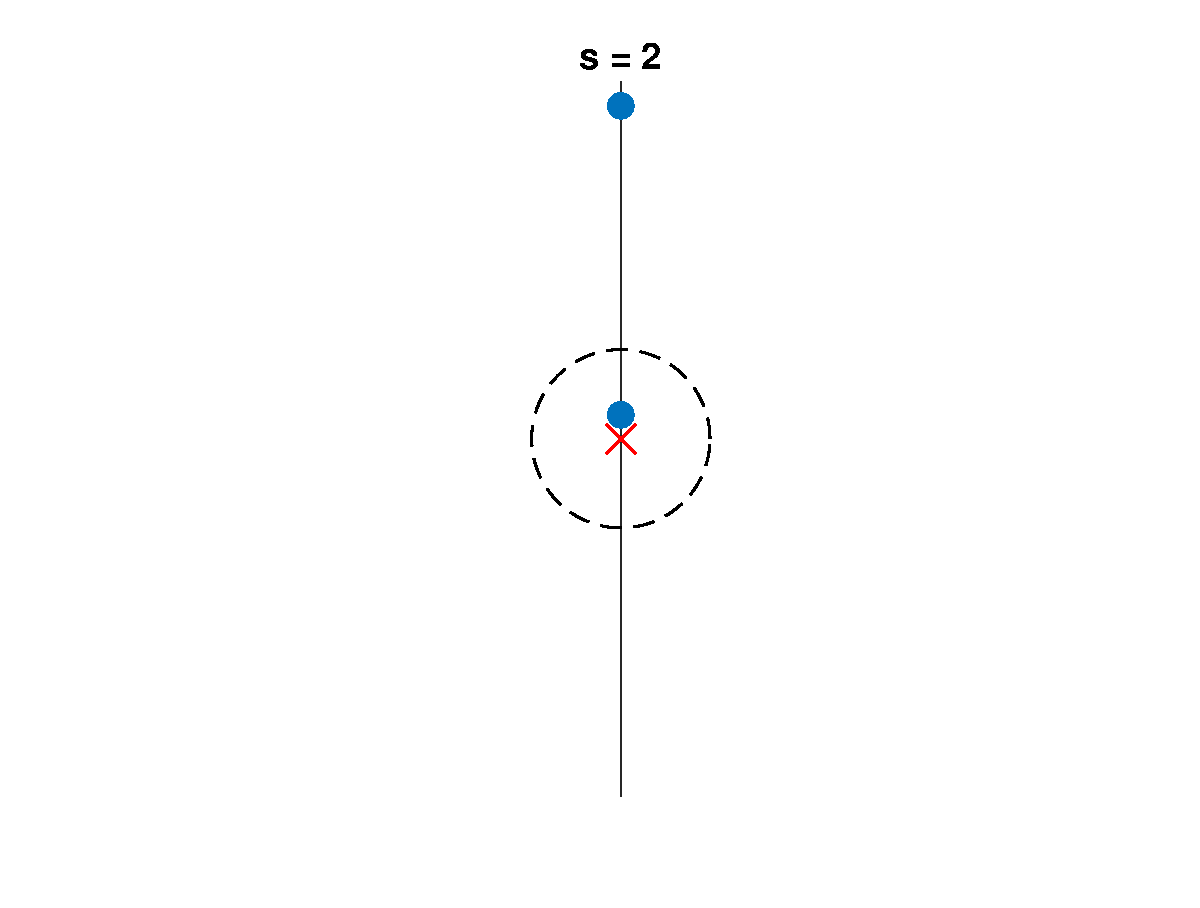
\includegraphics[width=5cm]{images/kreinbubbles/bubble2R} &
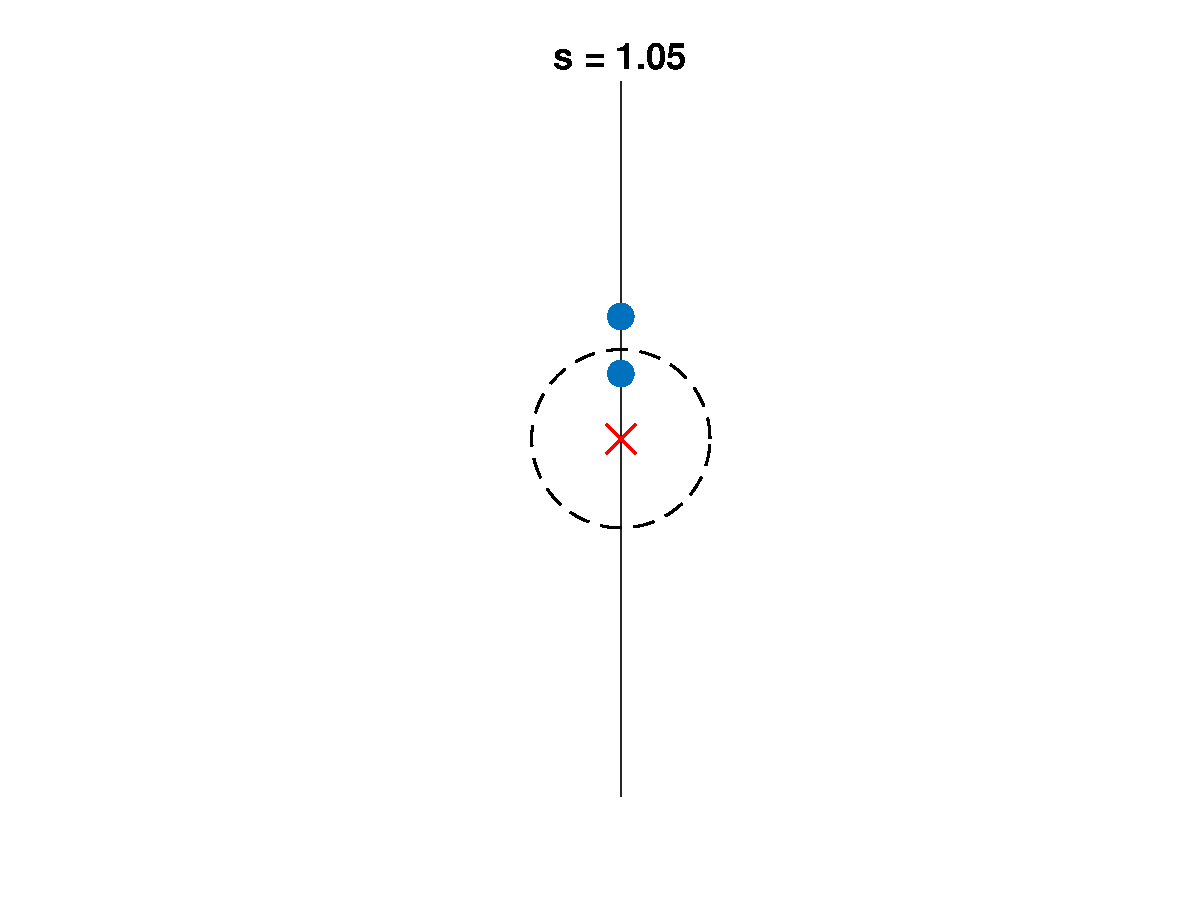
\includegraphics[width=5cm]{images/kreinbubbles/bubble105R} &
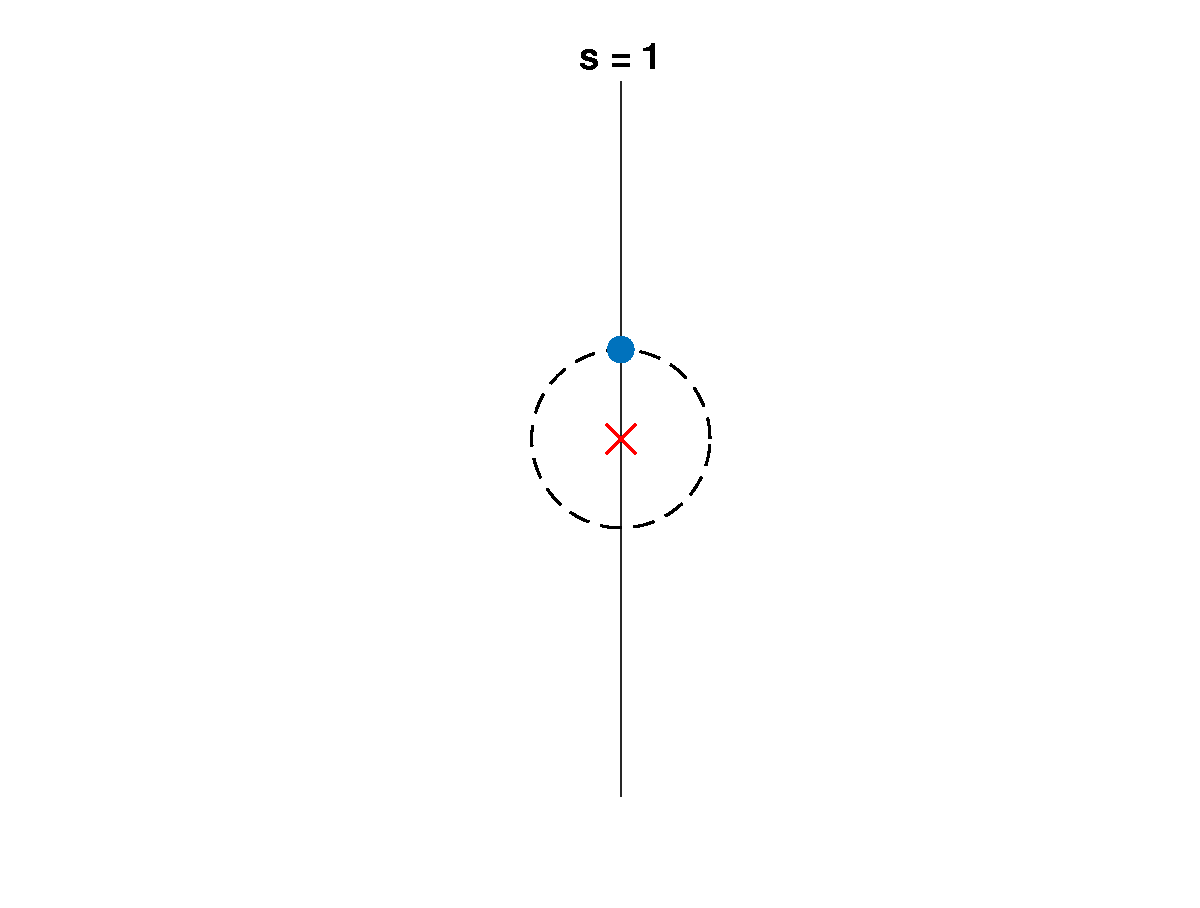
\includegraphics[width=5cm]{images/kreinbubbles/bubbleR} \\
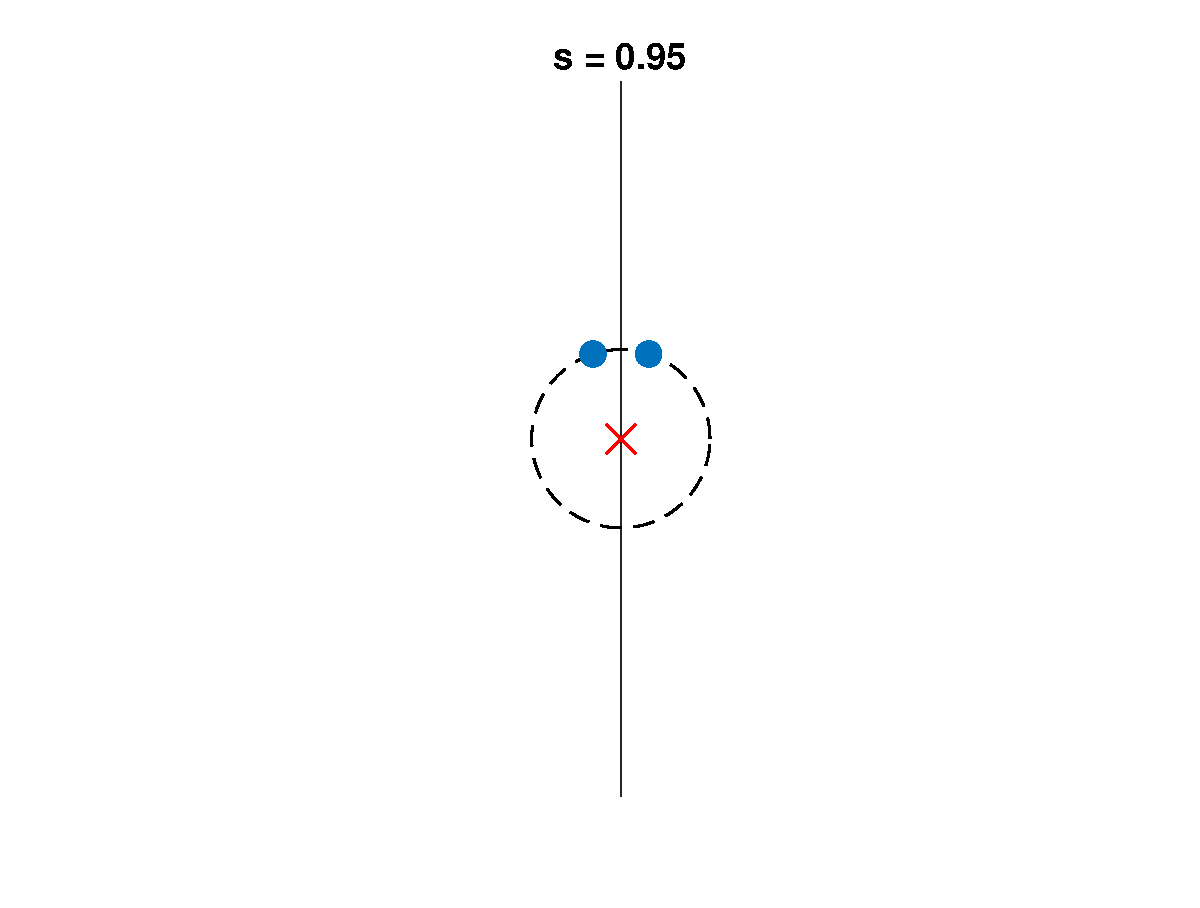
\includegraphics[width=5cm]{images/kreinbubbles/bubble095R} &
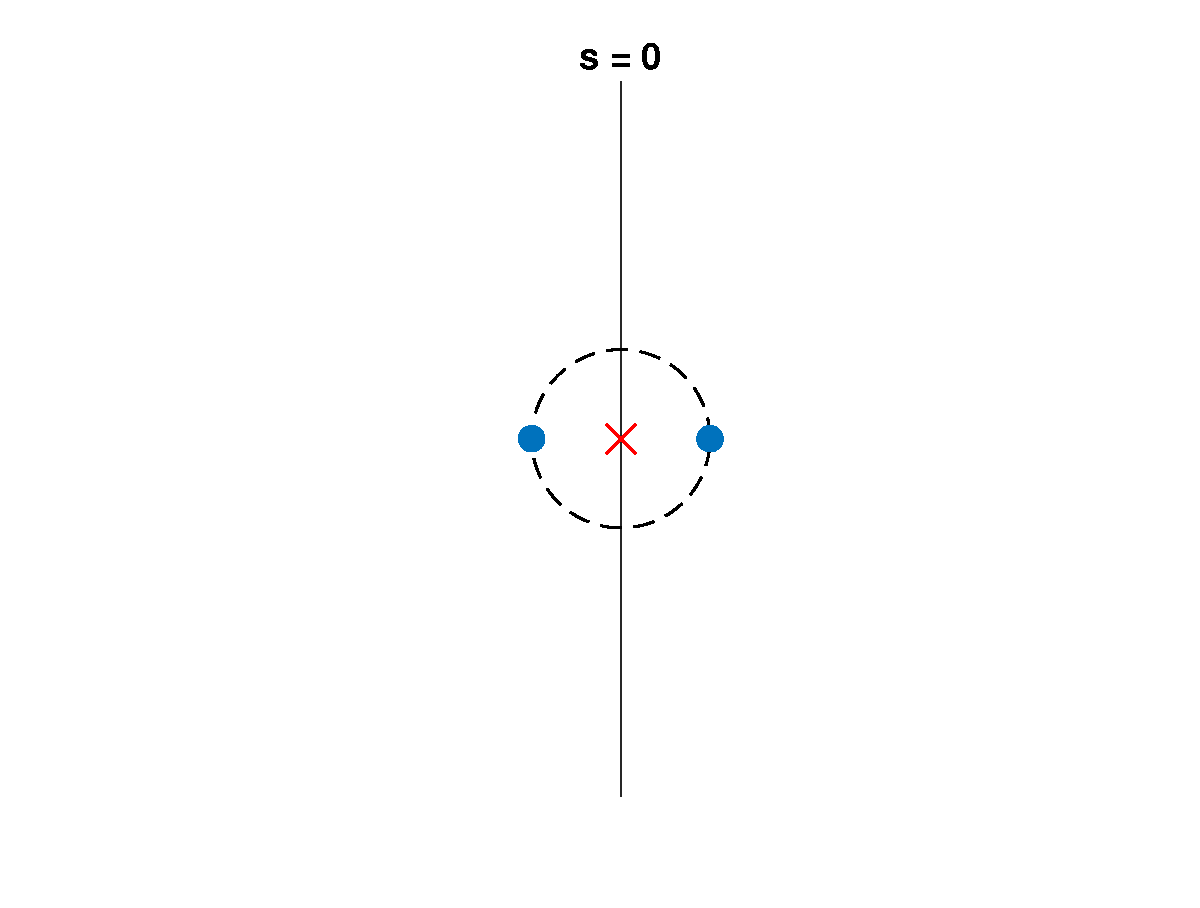
\includegraphics[width=5cm]{images/kreinbubbles/bubble0} &
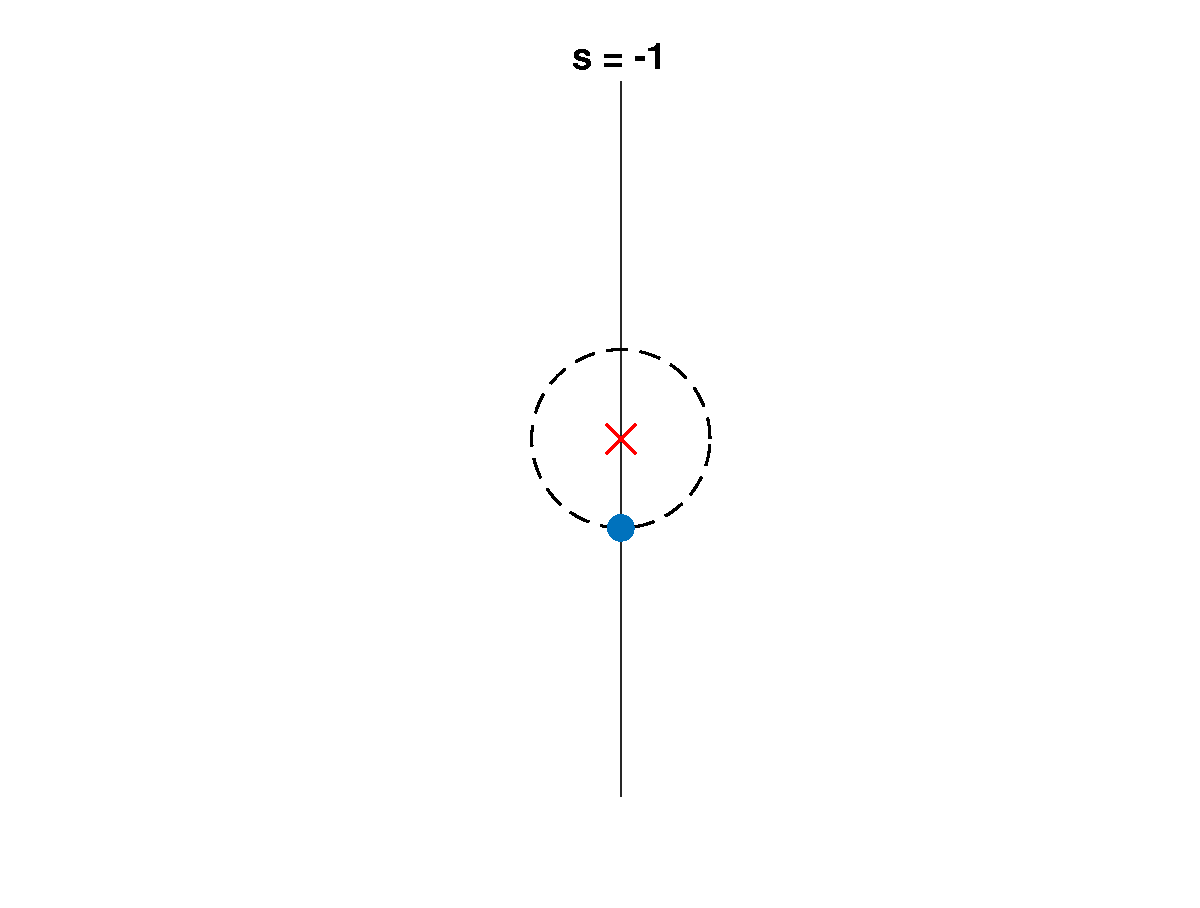
\includegraphics[width=5cm]{images/kreinbubbles/bubbleminusR}
\end{tabular}
\caption{Plot of the complex plane illustrating eigenvalue collision and Krein bubble as parameter $t$ is decreased. Blue dots are the pair of eigenvalues. Red cross is the point $\lambda_* i$. Vertical line is the imaginary axis. Black dotted circle is the circle of radius $\sqrt{R}$ around $\lambda_*$ }
\label{fig:kreinbubbles}
\end{center}
\end{figure}

We will call the instability bubble a Krein bubble, since it results from the collision of two imaginary eigenvalues with opposite Krein signatures. Inside the Krein bubble, the eigenvalues $\lambda_{1,2}$ are symmetric across the imaginary axis. Outside the Krein bubble, where $\lambda_{1,2}$ are purely imaginary, there is no such symmetry; Hamiltonian symmetry tells us instead that there exist eigenvalues $-\lambda_{1,2}$ which are in the lower half-plane.

In the following theorem, we prove that Krein bubbles occur. For simplicity, we will only consider the first Krein bubble, which occurs when an imaginary interaction eigenvalue collides with the first nonzero essential spectrum eigenvalue. The same analysis works for collisions with subsequent essential spectrum eigenvalues. To make this work, for $m_0 \in \{ 0, 1 \}$ and $s_0 > p^*$, let $Q_2(x; m_0, s_1, r)$ be the corresponding family of asymmetric periodic 2-pulses from Theorem \ref{2pulsebifurcation}. Using Theorem \ref{theorem:2peigsassym}, select whichever of $m_0 \in \{ 0, 1 \}$ will give us an interaction eigenvalue on the imaginary axis. Since for $s_1$ fixed, Krein bubbles do not occur for sufficiently small $r$, we will need $s_1$ and $r$. Using \cref{theorem:2peigsassym} as a guide, we wish to choose $s_1$ so that $c \pi/X$ is close to $\sqrt{\frac{2 \tilde{a}(r)}{M}}r^{1/2}$. The complication is that both $\tilde{a}(r)$ and $X$ depend on $s_1$ and $r$. By \cref{lemma:chara}, for small $r$ and large $s_1$, $\tilde{a}(0)$ is close to $\tilde{a}^*(m_0)$. In the next lemma, we show that we can always find an appropriate $s_1$.

\begin{lemma}\label{lemma:s1choice}
Let $\tilde{a}^*(m_0)$ be as in Lemma \ref{lemma:chara}, and choose $m_0 \in \{ 0, 1\}$ so that $\tilde{a}^*(m_0)/M > 0$. Let $r_*$ and $X(r, m_0, s_1)$ be as in \cref{theorem:2peigsassym}. Let
\begin{equation}\label{tildelambdastar}
\tilde{\lambda}_* = \sqrt{\frac{ 2 \tilde{a}^*(m_0) }{M}}
\end{equation}
Then there exists $r_1 \leq r_*$ such that for all $r \leq r_*$, there exists $s_1^*(r) > p^*$ such that
\begin{equation}\label{choosesstar}
\tilde{\lambda}_* r^{1/2} = \frac{c \pi}{X(r, m_0, s_1^*(r))}
\end{equation}
\end{lemma}

The following theorem then characterizes the Krein bubble.

\begin{theorem}\label{theorem:kreinbubbles}
Assume Hypotheses \ref{Ehyp}, \ref{Hhyp}, \ref{hypeqhyp}, \ref{Qexistshyp}, \ref{H0transversehyp}, and \ref{Melnikov2hyp}. Choose $m_0 \in \{0, 1\}$ as in Lemma \ref{choosesstar} and let $r_1$, $\tilde{\lambda}_*$, and $s^*(r)$ be as in Lemma \ref{choosesstar}. Choose $N = 1$ and let $\delta(r) = \delta(r,1)$, $M$ and $M^c$ be as in Theorem \ref{blockmatrixtheorem}. For $r \leq r_1$, let
\begin{enumerate}[(i)]
\item $X^*(r) = X(r, m_0, s_1^*(r))$ 
\item $X_0^*(r) = X_0(r, m_0, s_1^*(r))$
\item
$
\begin{aligned}[t]
R_0(r) = \frac{M^c q(X_0^*(r))}{M},
\end{aligned}
$
where $q(x)$ is the first component of the primary pulse $Q(x)$
\item
$
\begin{aligned}[t]
R(r) = \lambda_*(r)^2 R_0(r) \frac{X_0^*(r)}{X^*(r)}
\end{aligned}
$
\end{enumerate}

Then there exists $r_2 \leq r_1$ such that for all $r \leq r_2$, the following is true. Let $t \in [-2, 2]$. For $s_1 = s_1(r, t)$ close to $s_1^*(r)$, there exists a pair of eigenvalues located at
\begin{align*}
\lambda_{1,2}(t) = \left( \lambda_* + t \sqrt{R(r)} \right) i \pm \sqrt{(1 - t^2)R(r)} + \text{``h.o.t.''}
\end{align*}
WE CAN WRITE $s_1(r, t)$ AND $X(r)$ IN TERMS OF $t$. If $R_0(r) > 0$, these eigenvalues have the following configuration.
\begin{itemize}
\item For $|t| < 1$, $\lambda_{1,2}(t)$ is symmetric across the imaginary axis, i.e. $\lambda_2(t) = -\overline{\lambda_1}(t)$. For $t = 0$, these are given by
\[
\lambda_{1,2}(t) = \lambda_* i \pm (\sqrt{R(r)} + ``h.o.t.'')
\]
\item For $|r| \in (1, 2]$, $\lambda_{1,2}(r)$
are purely imaginary. For $r = 2$, one of $\lambda_{1,2}(r)$ is close to $\lambda_* i$.

\item At $t = \pm 1$, $\lambda_{1,2}(t)$ collide on the imaginary axis at 
\[
\lambda_{1,2}(t) = \lambda_* i \pm (\sqrt{R(r)} + ``h.o.t.'')
\]
\end{itemize}
For $|t| \leq 1$, the eigenvalues $\lambda_{1,2}(t)$ are, to leading order, located on a circle of radius $\sqrt{R(r)}$ about $\lambda_* i$ in the complex plane, where
\[
\sqrt{R(r)} = C r^{3/4}\frac{X_0^*(r)}{X^*(r)}
\]
\end{theorem}

\section{Spectrum of periodic multi-pulses}

We can state an analogue to \cref{theorem:2peigsassym} for periodic multi-pulses. For $n \geq 3$, it is not feasible to compute the determinant of the block matrix. To obtain a result, we will place an additional condition on the matrix $A$. We start with the following lemma, which in some ways is analogous to \cref{lemma:chara} but provides much less information.

\begin{lemma}\label{lemma:charmatrixA}
For any periodic parameterization $(m_0, \dots, m_{n-1}, \theta)$ with $\theta \notin \{-\pi + p^*, p^* \}$, let $r_* = r^*(m_0, \dots, m_{n-1}, \theta)$ be as in \cref{perexist}. Let $A$ be the matrix from \cref{blockmatrixtheorem}. Then for all $r \leq r_*$,
\[
A = r \tilde{A}(r)
\]
where $\tilde{A}(r) = \tilde{A}(r; m_0, \dots, m_{n-1}, \theta)$ is smooth in $r$. $\tilde{A}(r)$ has an eigenvalue of 0 corresponding to eigenvector $(1, 1, \dots, 1)^T$. 
\end{lemma}

Let $\{ 0, \ell_1(r), \dots, \ell_{n-1}(r) \}$ be the eigenvalues of $\tilde{A}(r)$. We will take the following hypothesis regarding these eigenvalues.

\begin{hypothesis}\label{Adistincteigs}
The eigenvalues $\{ 0, \ell_1(0), \dots, \ell_{n-1}(0)\}$ of $\tilde{A}(0)$ are distinct.
\end{hypothesis}
This hypothesis implies that $\tilde{A}(0)$ has a one-dimensional kernel. The eigenvalues of $\tilde{A}(0)$ only depend on the periodic parameterization $(m_0, \dots, m_{n-1}, \theta)$.

\begin{remark}
\cref{Adistincteigs} is not true in general. For example, if $n \geq 3$ and all of $m_j$ are the same, then $\tilde{A}(0)$ is a circulant matrix. It is not hard to show that $\tilde{A}(0)$ will have at least one eigenvalue of algebraic multiplicity 2.
\end{remark}

We can now state the following theorem. As we did in \cref{theorem:2peigsassym}, we will always choose $r$ sufficiently small so that the essential spectrum does not interfere.

\begin{theorem}\label{theorem:multieigs}
Assume Hypotheses \ref{Ehyp}, \ref{Hhyp}, \ref{hypeqhyp}, \ref{Qexistshyp}, \ref{H0transversehyp}, \ref{Melnikov2hyp}. Let $\tilde{A}(r)$ be as in \cref{lemma:charmatrixA}. Let $(m_0, \dots, m_{n-1}, \theta)$, with $\theta \notin \{-\pi + p^*, p^* \}$, be a periodic parameterization for which \cref{Adistincteigs} holds, and let $\{ 0, \ell_1(0), \dots, \ell_{n-1}(0)\}$ be the distinct eigenvalues of $\tilde{A}(0)$. 

Let $r_* = r_*(m_0, \dots, m_{n-1}, \theta)$ be as in \cref{perexist}. Choose any integer $N > 0$, and let $\delta(N,r)$ be as in Theorem \ref{blockmatrixtheorem}. Then there exists $r_1 = r_1(m_0, \dots, m_{n-1}, \theta, N) \leq r_*$ with the following property. For any $r \leq r_1$, the following hold regarding the spectrum associated with periodic multi-pulse $Q_2(x; m_0, \dots, m_{n-1}, \theta, r)$.

\begin{enumerate}[(i)]
\item There is an eigenvalue at 0 with algebraic multiplicity 3.
\item Let $N_1 \leq N$ be the largest positive integer such that $N_1/|\log r| < \delta(N,r)$. Then there are $2N_1$ nonzero essential spectrum eigenvalues $\lambda = \{ \pm \lambda_m^{\text{ess}} : m = 1, \dots, N_1 \}$, where
\[
\lambda_m^{\text{ess}}(r) = c \frac{m \pi i}{X}+  \mathcal{O}\left( \frac{1}{|\log r|^2} \right)
\]
is on the imaginary axis and $X = X(r; m_0, \dots, m_{n-1}, \theta)$ is given by \cref{Xdomain}.

\item There are $n - 1$ pairs of nonzero interaction eigenvalues located at
\begin{align*}
\lambda &= \pm \lambda^{\text{int}}_j(r) && j = 1, \dots, n-1,
\end{align*}
where
\begin{align*}
\lambda^{\text{int}}_j(r) = \sqrt{\frac{\ell_j(0)}{M}}r^{1/2} + \mathcal{O}\left( \frac{r^{1/2}}{|\log r|}\right)
\end{align*}
and $|\lambda^{\text{int}}_j(r)| < \frac{1}{2}|\lambda_1^{\text{ess}}(r)|$ for all $j$. The interaction eigenvalue pairs are either real or purely imaginary.

\item There are no other eigenvalues inside a circle with radius slightly larger than $|\lambda_{N_1}^{\text{ess}}(r)|$.

\end{enumerate}
\end{theorem}

For the periodic 2-pulse, the interaction eigenvalue pattern is determined by the sign of the nonzero eigenvalue of $\tilde{A}(0)$; this is given by \cref{lemma:chara}. For $n \geq 3$, there is no easy way to determine these signs. If $m_{n-1}$ is very large compared to the other $m_j$, the matrix $A$ is approximately the tri-diagonal matrix in \cite[Theorem 2]{Sandstede1998}. In principle, we could use a similar argument to \cite[Theorem 3(iv)]{Sandstede1998} to determine the interaction eigenvalue pattern in terms of the parity of the integers $m_0, \dots, m_{n-2}$. This is beyond the scope of this work.

\iffulldocument\else
	\bibliographystyle{amsalpha}
	\bibliography{thesis.bib}
\fi

\end{document}